
\mychapter{State Estimation}{State Estimation}{}
\label{chap:stateestimation}

%==================================================================================================================================================================================
\mysection{Introduction}{Introduction}
\label{sec:stateintro}

After modeling the satellite and sensors in Chapter 3, and designing the Earth Tracker in Chapter 4, Chapter 5 now focuses on the estimator. The chapter 
begins with a basic background on recursive estimators, followed by a detailed discussion of the Kalman Filter. Next, the system modeling within the pose estimator is 
presented, starting with the motion model and then the measurement models. The Earth Tracker measurement model is addressed first, followed by the supporting sensor 
measurement models. Finally, the chapter concludes with a description of the system initialization and design.

%=========================================================================================================================================================================
\mysection{Recursive Estimation}{Recursive Estimation}
\label{sec:stateEKF}

This section introduces the concept of recursive estimators and highlights several commonly used approaches in localization and tracking. A recursive 
estimator updates the current state distribution by combining the prior distribution of the system states with the latest sensor measurements. The 
basic operation of a discrete recursive filter is illustrated in Figure \ref{fig:RE} \cite{Jiang}.

\begin{figure}[H]
    \centering
    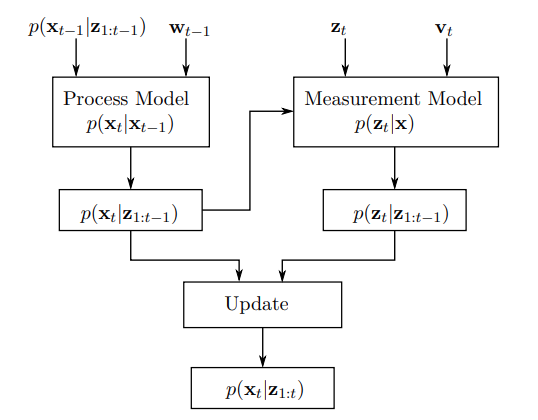
\includegraphics[width=0.6\linewidth]{figures/StateEstimation/Recursive Estimation.png}
    \caption{Recursive estimator algorithm flowchart \cite{deJongh2019}}
    \label{fig:RE}
\end{figure}

\noindent
The system state at time $t$ is represented by $\mathbf{x}_t$ in the discrete time domain. The process, or state transition function, is expressed as

\begin{equation}
    \mathbf{x}_t = \mathbf{f}(\mathbf{x}_{t-1},\mathbf{u}_{t-1},\mathbf{w}_{t-1})
\end{equation}

\noindent
where $\mathbf{f}$ is either a linear or non-linear transition function, $\mathbf{u}_{t-1}$ represents the control input, and $\mathbf{w}_{t-1}$ represents the process 
noise. New observations $\mathbf{z}_t$ are available at discrete timesteps and are related to the system state by the measurement function

\begin{equation}
    \mathbf{z}_t = \mathbf{h}(\mathbf{x}_t,\mathbf{v}_t)
\end{equation}

\noindent
where $\mathbf{h}$ is the observation model and $\mathbf{v}_t$ is the measurement noise. The goal is to obtain the
posterior distribution, $p(\mathbf{x}_t|\mathbf{z}_{1:t})$, over the state vector $\mathbf{x}_t$. This is done by recursively performing process and measurement updates.
\vspace{0.5cm}

\noindent
At a time $t$, the posterior distribution over $\mathbf{x}_{t-1}$ is assumed to be known. The prior distribution at $t$ is then calculated as

\begin{equation}
    p(\mathbf{x}_t|\mathbf{z}_{1:t-1}) = \int p(\mathbf{x}_t|\mathbf{x}_{t-1})p(\mathbf{x}_{t-1}|\mathbf{z}_{1:t-1})\ \cdot d\mathbf{x}_{t-1} \text{.}
\end{equation}

\noindent
The measurement update is used to calculate the new posterior at time $t$, given the prior state distribution, according to Bayes' rule,

\begin{equation}
    p(\mathbf{x}_t|\mathbf{z}_{1:t}) = 
    \frac{p(\mathbf{z}_t|\mathbf{x}_t)p(\mathbf{x}_t|\mathbf{z}_{1:t-1})}{p(\mathbf{z}_t|\mathbf{z}_{1:t-1})} \text{.}
\end{equation}

\noindent
The Kalman Filter is a popular estimator used in pose estimation problems. It is a special case of the Bayes filter, where Gaussian noise distributions are assumed.
The initial system distribution is also assumed Gaussian. A control and measurement update is executed
at each sampling instant to update the distribution over the states. If the previous state distribution is Gaussian, then the updated current distribution will also be Gaussian,
and therefore the best estimate, $\hat{\mathbf{x}}_t$, is chosen as the mean of the distribution. Different variants of the Kalman Filter exist, of which the 
Extended and Unscented Kalman Filters are the most popular.
\vspace{0.5cm} 

\noindent
The Extended Kalman Filter (EKF) overcomes the restrictions of the linear filter by approximating non-linear functions to be linear using a first-order Taylor expansion.
The mean of the state distribution is used as the linearisation point around which the tangent of the non-linear function is calculated, allowing the use of standard
Kalman Filter equations. It is typically more efficient than other non-linear filters, sometimes at the cost of reduced accuracy.
\vspace{0.5cm}

\noindent
The Unscented Kalman Filter (UKF) uses stochastic linearisation to deal with non-linear systems. Given a distribution with a known mean and covariance, a set of weighted points,
known as sigma points, are chosen and transformed using the non-linear function. A new distribution is determined from the transformed sigma points. The process and observation
functions do not need to be differentiable and the output is based on values in a larger region, rather than a local approximation.
\vspace{0.5cm}

\noindent
In this context, the EKF is preferred due to its balance between computational efficiency and estimation accuracy. While the UKF provides improved handling of strong nonlinearities, the EKF remains well suited for systems where the nonlinear behaviour is moderate and the dynamics can be reliably linearised around the current estimate, which typically applies in attitude or pose estimation problems. Furthermore, the EKF's reliance on analytical Jacobians offers greater transparency and control over the estimation process, which is beneficial for interpreting results and diagnosing model behaviour. Its relatively low computational cost makes it attractive for real-time implementations or onboard processing, where resources are limited but estimation accuracy must still be maintained.

%===============================================================================================================================================================================
\mysection{The Extended Kalman Filter}{The Extended Kalman Filter}

Kalman filters are well suited for localistation problems since the nature of these systems are normally non-linear. Both the linear and non-linear variants of the Kalman Filter
are concerned with estimating states using a motion model and is able to perform measurement fusion. The state estimation problem in this work makes use of non-linear system 
models, and a high-dimensinal state space. The EKF is well suited for this problem, since it accomodates non-linear process and observation models and is capable 
of dealing with high-dimensional state spaces. The EKF is often use for the Simultaneous Localisation and Mapping (SLAM) problem and is well known in the field of robotics and localisation. The EKF is governed by the following set of equations, as presented in Section \ref{sec:Prediction} - \ref{sec:MSE} and further described in \cite{Alex}.
\vspace{0.5cm}

%==========================================================================================================================================================
\mysubsection{The Prediction Step}{The Prediction Step}
\label{sec:Prediction}

The prediction step, also known as the time update, projects the current state and error covariance estimates forward to obtain the estimates for the next time step. 
This is defined as follows:

\begin{equation}
    \mathbf{\hat{x}}_{t+1,t} = \mathbf{f}(\mathbf{\hat{x}}_{t,t}) + \mathbf{G}\mathbf{u}_t \text{, and}
\end{equation}

\begin{equation}
    \mathbf{P}_{t+1,t} = \mathbf{F}_t\mathbf{P}_{t,t}\mathbf{F}_t^T + \mathbf{Q}
    \label{Eq:P}
\end{equation}

\noindent
where $\mathbf{\hat{x}}$ represents the estimated state, $\mathbf{f}$ is the process model of the system, $\mathbf{G}$ is the control matrix, and $\mathbf{u}$ is the control input. 
The term $\mathbf{P}$ is the state covariance matrix, which represents the uncertainty of each state. $\mathbf{F}$ is the Jacobian of the process model, and $\mathbf{Q}$ is the 
process noise covariance matrix. This final matrix, shown in Eqaution \ref{Eq:P}, represents the uncertainty in the process model itself, accounting for discrepancies between the mathematical model and the 
true physical system.
\vspace{0.5cm}

\noindent
Since the motion model, $\mathbf{f}$, is a non-linear vector function, it must be linearized at each time step to apply the standard Kalman Filter equations for covariance 
propagation. The function is linearized around the most recent state estimate, $\mathbf{\hat{x}}_{t,t}$, using a first-order Taylor series expansion:

\begin{equation}
    \mathbf{f}(\mathbf{\hat{x}}) \approx \mathbf{f}(\mathbf{\hat{x}}_{t,t}) + \mathbf{F}_t(\mathbf{\hat{x}}-\mathbf{\hat{x}}_{t,t})
\end{equation}

\noindent
where $\mathbf{F}_t$ is the Jacobian matrix of the process model, evaluated at the current state estimate $\mathbf{\hat{x}}_{t,t}$:

\begin{equation}
  \begin{aligned}
    \mathbf{F}_t = \mathbf{F}(\mathbf{\hat{x}}_{t,t})
     &= \left. \frac{\partial \mathbf{f}(\mathbf{\hat{x}})}{\partial \mathbf{\hat{x}}} \right|_{\mathbf{\hat{x}} = \mathbf{\hat{x}}_{t,t}} \\
     &=
    \begin{bmatrix}
      \dfrac{\partial f_1}{\partial \hat{x}_1} & \cdots & \dfrac{\partial f_1}{\partial \hat{x}_n} \\
      \vdots & \ddots & \vdots \\
      \dfrac{\partial f_m}{\partial \hat{x}_1} & \cdots & \dfrac{\partial f_m}{\partial \hat{x}_n}
    \end{bmatrix}
  \end{aligned}
\end{equation}
\vspace{0.5cm}

\noindent
The required partial derivatives for the Jacobian are approximated using midpoint numerical differentiation, expressed as:

\begin{equation}
f'(x) \approx \frac{f(x+e)-f(x-e)}{2e}
\end{equation}

\noindent
where $e$ denotes a small perturbation applied in both directions to evaluate the gradient. Although a symbolic solution for the Jacobian is theoretically possible, 
preliminary tests showed that it is computationally expensive and thus impractical for real-time implementation.

%============================================================================================================================================================
\mysubsection{The Update Step}{The Update Step}
\label{sec:Update}

The update step, also known as the measurement update, corrects the state estimate from the prediction step using a new measurement from a sensor. This process 
refines the estimate and reduces its uncertainty. The step begins by computing the difference between the actual measurement and the predicted measurement.
\vspace{0.5cm}

\noindent
First, the innovation or measurement residual, $\mathbf{y}_t$, is computed. This represents the new information available to the filter, which is the discrepancy between the actual 
sensor measurement and the predicted measurement:

\begin{equation}
    \mathbf{y}_t = \mathbf{z}_t - \mathbf{h}(\mathbf{\hat{x}}_{t,t-1})
\end{equation}

\noindent
where \(\mathbf{z}_t\) is the actual measurement vector and \(\mathbf{h}(\cdot)\) is the non-linear measurement model that maps the state space into the measurement space.
\vspace{0.5cm}

\noindent
Next, the innovation covariance, $\mathbf{S}_t$, is calculated. It represents the total uncertainty of the innovation, combining the uncertainty of the predicted state 
and the measurement noise:

\begin{equation}
    \mathbf{S}_t = \mathbf{H}_t\mathbf{P}_{t,t-1}\mathbf{H}_t^T + \mathbf{R}_t
\end{equation}

\noindent
where $\mathbf{H}_t$ is the Jacobian of the measurement model $\mathbf{h}$ evaluated at the  state estimate $\mathbf{\hat{x}}_{t,t-1}$, and $\mathbf{R}_t$ 
is the measurement noise covariance matrix.
\vspace{0.5cm}

\noindent
Using the innovation covariance, the optimal Kalman Gain, \(\mathbf{K}_t\), is computed. The gain determines the weight given to the innovation when updating the state estimate:

\begin{equation}
    \mathbf{K}_t = \mathbf{P}_{t,t-1}\mathbf{H}_t^T \mathbf{S}_t^{-1}
\end{equation}

\noindent
Finally, the state estimate and its covariance are corrected using the Kalman Gain and the innovation to produce the final, more accurate estimates for the 
current time step.

\begin{equation}
    \mathbf{\hat{x}}_{t,t} = \mathbf{\hat{x}}_{t,t-1} + \mathbf{K}_t \mathbf{y}_t
\end{equation}

\noindent
The state covariance is updated to reflect the reduction in uncertainty resulting from the measurement. The Joseph form of the covariance update equation, chosen for its
numerical stability, is used:

\begin{equation}
    \mathbf{P}_{t,t} = (\mathbf{I}-\mathbf{K}_t\mathbf{H}_t)\mathbf{P}_{t,t-1}(\mathbf{I}-\mathbf{K}_t\mathbf{H}_t)^T + \mathbf{K}_t\mathbf{R}_t\mathbf{K}_t^T
\end{equation}

\noindent
where \(\mathbf{I}\) is the identity matrix.

%===================================================================================================================================================================
\mysubsection{Multi-Sensor Fusion Techniques}{Multi-Sensor Fusion Techniques}
\label{sec:MSE}

EKFs can combine information from multiple sensors in several different ways. Three common fusion strategies are outlined below:
\vspace{0.5cm}

\noindent
\textbf{Batch EKF}\\
In a batch EKF, all sensor models are combined into a single filter that directly fuses raw measurements. This “fully integrated” approach can be 
more optimal because it explicitly accounts for cross-correlations between the different sensor measurements. However, it is computationally more 
demanding and may become impractical for systems with many heterogeneous sensors.

\begin{figure}[H]
    \centering
    \includegraphics[width=0.7\linewidth]{figures/stateestimation/EKFComplexModel.pdf}
    \caption{The fully integrated Batch EKF architecture, which combines all raw sensor data into a single, complex measurement model $\mathbf{h}(\mathbf{x})$ for concurrent processing.}
    \label{fig:EKFCM}
\end{figure}

\noindent
\textbf{Multi-Filter EKF}\\
In a multi-filter EKF, each sensor (or group of sensors) maintains its own local EKF. A higher-level master filter then fuses these local estimates 
into a global state. This approach is modular and makes fault isolation easier, but it requires careful handling of inter-filter correlations and can 
introduce additional latency.

\begin{figure}[H]
    \centering
    \includegraphics[width=\linewidth]{figures/stateestimation/EKFMaster.pdf}
    \caption{The Multi-Filter EKF architecture, featuring independent local filters for each sensor and a master filter to fuse the local estimates into a global state.}
    \label{fig:EKFM}
\end{figure}

\noindent
\textbf{Sequential Update EKF}\\
In the sequential update approach, a single EKF processes sensor measurements one at a time rather than combining them into a single batch. 
This is essentially the standard EKF formulation: a prediction step is followed by multiple updates, each corresponding to one sensor measurement. 
This method is particularly useful for systems with asynchronous sensors operating at different sampling rates.

\begin{figure}[H]
    \centering
    \includegraphics[width=0.6\linewidth]{figures/stateestimation/EKFSequencial.pdf}
    \caption{The Sequential Update EKF architecture, illustrating a single prediction step followed by multiple, sequential update steps for each individual sensor measurement.}
    \label{fig:EKFS}
\end{figure}

\noindent
In this work, the sequential update EKF is adopted, as it aligns well with the characteristics of satellite sensor suites. For instance, 
GPS measurements are relatively slow but absolute, while gyroscopes provide high-frequency angular velocity data that drift over time. Star trackers 
deliver highly accurate orientation information, though at lower update rates. Coarse sun sensors and magnetometers supply additional measurements 
that are less accurate but robust and continuously available. Processing these measurements sequentially allows the filter to integrate information at 
the rate each sensor provides it.
\vspace{0.5cm}

\noindent
It is important to note that the order of updates in the sequential approach affects the filter's performance. A common strategy is to process measurements 
from lower-accuracy or noisier sensors first (e.g., coarse sun sensor, magnetometer), followed by higher-accuracy sensors such as the star tracker. 
This ensures that the state estimate is progressively refined rather than being skewed or “pulled” away from the true value by noisier updates.

%===============================================================================================================================================================================
\mysection{System Modelling}{System Modelling}
\label{sec:statesystemmodel}

The system states are defined as,

\begin{equation}
    \mathbf{\hat{x}}_t =
    \begin{bmatrix}
        \mathbf{\hat{r}}_\mathcal{I} & \mathbf{\hat{v}}_\mathcal{I} & \mathbf{\hat{q}}_\mathcal{B/O} & \boldsymbol{\hat{\omega}}_\mathcal{B/O}^\mathcal{B}
    \end{bmatrix}
    ^T
\end{equation}

\noindent
Figure \ref{fig:System Modelling} illustrates the state variables defined within the Earth-Centered Inertial (ECI) reference frame. The terms $ \mathbf{r}_\mathcal{I} $ and
$ \mathbf{v}_\mathcal{I} $ represent the satellite's position and velocity in the ECI frame, respectively. The attitude of the satellite's Body frame relative to the Orbital 
reference frame is denoted by $ \mathbf{q}_\mathcal{B/O} $, while the angular velocity of the Body frame relative to the Orbital frame, expressed in Body coordinates, 
is denoted by $ \boldsymbol{\omega}_\mathcal{B/O}^\mathcal{B} $.

\begin{figure}[H]
    \centering
    \includegraphics[width=0.8\textwidth]{figures/stateestimation/OverallSystem.pdf}
    \caption{Satellite pose estimation states in the ECI reference frame}
    \label{fig:System Modelling}
\end{figure}

%============================================================================================================================================================================
\mysubsection{Motion Model}{Motion Model}
\label{sec:statemotionmodel}

The rotation of the satellite body is non-linear and the satellite motion from one timestep to the next when using Newton-Euler coupling can be described by the motion model
$\mathbf{f}$,

\begin{equation}
    \mathbf{\hat{x}}_t = \mathbf{f}(\mathbf{x}_{t-1},\mathbf{u}_t)
\end{equation}

\noindent
which is expanded to,

\begin{equation}
    \mathbf{\hat{x}}_t
    =
    \begin{bmatrix}
        r_{x,t} \\
        r_{y,t} \\
        r_{z,t} \\
        v_{x,t} \\
        v_{y,t} \\
        v_{z,t} \\
        q_{s,t} \\
        q_{x,t} \\
        q_{y,t} \\
        q_{z,t} \\
        \omega_{x,t} \\
        \omega_{y,t} \\
        \omega_{z,t} \\
    \end{bmatrix}
    = \mathbf{\hat{x}}_{t-1} +
    \begin{bmatrix}
        v_{x,t-1} \\
        v_{y,t-1} \\
        v_{z,t-1} \\
        -\frac{\mu}{|\mathbf{r}|^3}\cdot r_{x,t-1} + a_{\text{J2},x,t-1} \\
        -\frac{\mu}{|\mathbf{r}|^3}\cdot r_{y,t-1} + a_{\text{J2},y,t-1} \\
        -\frac{\mu}{|\mathbf{r}|^3}\cdot r_{z,t-1} + a_{\text{J2},z,t-1} \\
        \frac{1}{2}(-\omega_{x,t-1}q_{x,t-1} - \omega_{y,t-1}q_{y,t-1} - \omega_{z,t-1}q_{z,t-1}) \\
        \frac{1}{2}( \omega_{x,t-1}q_{s,t-1} + \omega_{z,t-1}q_{y,t-1} - \omega_{y,t-1}q_{z,t-1}) \\
        \frac{1}{2}( \omega_{y,t-1}q_{s,t-1} - \omega_{z,t-1}q_{x,t-1} + \omega_{x,t-1}q_{z,t-1}) \\
        \frac{1}{2}( \omega_{z,t-1}q_{s,t-1} + \omega_{y,t-1}q_{x,t-1} - \omega_{x,t-1}q_{y,t-1}) \\
        \frac{1}{\mathit{I}_{xx}}(\mathit{I}_{yy}-\mathit{I}_{zz})\omega_{y,t-1}\omega_{z,t-1} \\
        \frac{1}{\mathit{I}_{yy}}(\mathit{I}_{zz}-\mathit{I}_{xx})\omega_{z,t-1}\omega_{x,t-1} \\
        \frac{1}{\mathit{I}_{zz}}(\mathit{I}_{xx}-\mathit{I}_{yy})\omega_{x,t-1}\omega_{y,t-1}
    \end{bmatrix}
    \Delta t + 
    \begin{bmatrix}
        0 \\
        0 \\
        0 \\
        0 \\
        0 \\
        0 \\
        0 \\
        0 \\
        0 \\
        0 \\
        \mathit{T}_x/\mathit{I}_x \\
        \mathit{T}_y/\mathit{I}_y \\
        \mathit{T}_z/\mathit{I}_z
    \end{bmatrix}
\end{equation}

\noindent
The body-fixed axes of the target are chosen to coincide with its principle axes of inertia. The principle moment of inertia are given as,

\begin{equation}
    \mathbf{I}_\mathcal{B} = 
    \begin{bmatrix}
        \mathit{I}_{xx} & 0 & 0 \\
        0 & \mathit{I}_{yy} & 0 \\
        0 & 0 & \mathit{I}_{zz}
    \end{bmatrix}
\end{equation}

\noindent
External torques, $\mathit{T}_x$, $\mathit{T}_y$ and $\mathit{T}_z$, within the model are asssumed to be zero and there is thus no control input, $\mathbf{u}_t$. 
\vspace{0.5cm}

\noindent
Thus 

\begin{equation}
    \mathbf{\hat{x}}_t = \mathbf{f}(\mathbf{x}_{t-1})
\end{equation}

\noindent
where

\begin{equation}
    \mathbf{\hat{x}}_t
    =
    \begin{bmatrix}
        r_{x,t} \\
        r_{y,t} \\
        r_{z,t} \\
        v_{x,t} \\
        v_{y,t} \\
        v_{z,t} \\
        q_{s,t} \\
        q_{x,t} \\
        q_{y,t} \\
        q_{z,t} \\
        \omega_{x,t} \\
        \omega_{y,t} \\
        \omega_{z,t} \\
    \end{bmatrix}
    = \mathbf{\hat{x}}_{t-1} +
    \begin{bmatrix}
        v_{x,t-1} \\
        v_{y,t-1} \\
        v_{z,t-1} \\
        -\frac{\mu}{|\mathbf{r}|^3}\cdot r_{x,t-1} + a_{\text{J2},x,t-1} \\
        -\frac{\mu}{|\mathbf{r}|^3}\cdot r_{y,t-1} + a_{\text{J2},y,t-1} \\
        -\frac{\mu}{|\mathbf{r}|^3}\cdot r_{z,t-1} + a_{\text{J2},z,t-1} \\
        \frac{1}{2}(-\omega_{x,t-1}q_{x,t-1} - \omega_{y,t-1}q_{y,t-1} - \omega_{z,t-1}q_{z,t-1}) \\
        \frac{1}{2}( \omega_{x,t-1}q_{s,t-1} + \omega_{z,t-1}q_{y,t-1} - \omega_{y,t-1}q_{z,t-1}) \\
        \frac{1}{2}( \omega_{y,t-1}q_{s,t-1} - \omega_{z,t-1}q_{x,t-1} + \omega_{x,t-1}q_{z,t-1}) \\
        \frac{1}{2}( \omega_{z,t-1}q_{s,t-1} + \omega_{y,t-1}q_{x,t-1} - \omega_{x,t-1}q_{y,t-1}) \\
        \frac{1}{\mathit{I}_{xx}}(\mathit{I}_{yy}-\mathit{I}_{zz})\omega_{y,t-1}\omega_{z,t-1} \\
        \frac{1}{\mathit{I}_{yy}}(\mathit{I}_{zz}-\mathit{I}_{xx})\omega_{z,t-1}\omega_{x,t-1} \\
        \frac{1}{\mathit{I}_{zz}}(\mathit{I}_{xx}-\mathit{I}_{yy})\omega_{x,t-1}\omega_{y,t-1}
    \end{bmatrix}
    \Delta t
    \label{Eq:StateTransition}
\end{equation}

\noindent
Equation \ref{Eq:StateTransition} illustrates that the position $\mathbf{r}_\mathcal{I}$ of the satellite only depends on the velocity $\mathbf{v}_\mathcal{I}$, whereas
the velocity depends on the acceleration, defined by the Newton-Euler equation. The acceleration of the model is composed of the gravitional accelaration $\mathbf{a}_\text{G}$ and the
$\mathbf{a}_{\text{J2}}$ which both where defined in Section \ref{sec:dynamics}. The attitude of the satellite is determined by the quaternion dynamic equation defined in Equation \ref{Eq:3.12}
and the angular velocity is defined with principle axis coupling.

%====================================================================================================================================================
\mysubsection{Sensor Measurement Model}{Sensor Measurement Model}

This section parallels Section~\ref{sec:SensorModelling}. While the earlier section constructed the measurement equations 
from the true satellite states, here the focus shifts to the \emph{estimated} states. These provide the basis for predicting 
sensor measurements within the Extended Kalman Filter (EKF). The predicted outputs $\hat{\mathbf{z}}$ are then compared to 
the actual noisy measurements $\mathbf{z}$ to form the innovation $\mathbf{\hat{y}}$.
\vspace{0.5cm}

\noindent
In general, each sensor measurement model can be written as

\begin{equation}
    \hat{\mathbf{z}} = \mathbf{h}(\hat{\mathbf{x}}_t),
\end{equation}

\noindent
where $\hat{\mathbf{x}}_t$ is the current state estimate. Since $\mathbf{h}(\cdot)$ is nonlinear, it is linearised about 
$\hat{\mathbf{x}}_t$ to obtain the measurement Jacobian

\begin{equation}
    \mathbf{H}_t = \frac{\partial \mathbf{h}}{\partial \mathbf{x}} \Big|_{\hat{\mathbf{x}}_t}.
\end{equation}

\noindent
The resulting Jacobian is used in the EKF update step. The following subsections summarise the sensor-specific forms of 
$\mathbf{h}(\hat{\mathbf{x}}_t)$.

%=========================================================================================================================================================================
\mysubsubsection{Earth Tracker Measurement Model}{Earth Tracker Measurement Model}

The Earth Tracker sends two inputs to the EKF, the measurement of the Earth Tracker itself 

\begin{equation}
    \mathbf{z}_{ET} = \mathbf{f}_\mathcal{B} =
    \begin{bmatrix}
        x_\mathcal{B} \\
        y_\mathcal{B} \\
        z_\mathcal{B}
    \end{bmatrix}
\end{equation}

\noindent
and the geolocated feature vector through the catalogue generation described in Section \ref{sec:CatalogueGeneration} also refered to as the catalogue vector 
$\mathbf{p}_\text{LLA}$.
\vspace{0.5cm}

\noindent
To transform this vector into a vector to be compared to the measurement, the following transformations are used

\begin{equation}
    \mathbf{f}_\mathcal{R} = f(\mathbf{p}_\text{LLA},WGS84)
\end{equation}

\noindent
and

\begin{equation}
    \mathbf{\hat{f}}_\mathcal{B}^+ = \mathbf{\hat{T}}_{\mathcal{O},t}^\mathcal{B} \times \mathbf{\hat{T}}_{\mathcal{I},t}^\mathcal{O} \times \mathbf{\hat{T}}_{\mathcal{R},t}^\mathcal{I} \times \mathbf{f}_\mathcal{R}^+
    \label{Eq:CatalogueH2}
\end{equation}

\noindent
where $\mathbf{\hat{T}}_{\mathcal{O},t}^\mathcal{B}$ is calculated using the estimated state $\mathbf{\hat{q}}_\mathcal{B/O}$, $\mathbf{\hat{T}}_{\mathcal{I},t}^\mathcal{O}$ is
calculated using the estimated state $\mathbf{\hat{r}}_\mathcal{I}$ and $\mathbf{\hat{v}}_\mathcal{I}$, and $\mathbf{\hat{T}}_{\mathcal{R},t}^\mathcal{I}$ is calculated by the 
rotation speed of the Earth $\omega_e$. This is done for each for each feature vector measurement, where the estimated Earth Tracker measurement is defined as:

\begin{equation}
    \mathbf{\hat{z}}_\text{ET} = \mathbf{\hat{f}}_\mathcal{B} = \mathbf{h}(\mathbf{\hat{x}}_t,\mathbf{p}_\text{LLA},\text{WGS84})\text{.}
\end{equation}

%====================================================================================================================================================
\mysubsubsection{GPS Measurement Model}{GPS Measurement Model}
\label{sec:GPSMeasModel}

\noindent 
The GPS receiver outputs measurements in geodetic coordinates $(\phi, \lambda, h)$ (latitude, longitude, and altitude). 
These must first be transformed into the Earth-Centered Earth-Fixed (ECEF) frame $\mathcal{R}$ from the ECI frame $\mathcal{I}$ 
using the estimated state information. The predicted GPS measurement is therefore expressed as

\begin{equation}
    \mathbf{\hat{r}}_{\mathcal{R}}^+ = \mathbf{\hat{T}}_{\mathcal{I},t}^\mathcal{R} \times \mathbf{\hat{r}}_{\mathcal{I}}^+
\end{equation}

\begin{equation}
    \mathbf{\hat{z}}_{\text{GPS}} = f(\mathbf{\hat{r}}_{\mathcal{R}},\text{WGS84})
\end{equation}

\begin{equation}
    \mathbf{\hat{z}}_{\text{GPS}} = \mathbf{h}_{\text{GPS}}(\mathbf{\hat{x}}_t,\text{WGS84}),
\end{equation}

\noindent where $\mathbf{\hat{r}}_\mathcal{I}$ is the estimated position vector in the inertial frame and 
$\mathbf{\hat{T}}_{\mathcal{I},t}^\mathcal{R}$ is the transformation from ECI to ECEF at time $t$. 
The WGS84 reference model is used for the ECEF-to-geodetic conversion.

%=====================================================================================================================================================
\mysubsubsection{Gyroscope Measurement Model}{Gyroscope Measurement Model}
\label{sec:GyroMeasModel}

\noindent The gyroscope measures the angular velocity of the body frame relative to the inertial frame, expressed in the body frame, 
denoted as $\boldsymbol{\omega}^\mathcal{B}_\mathcal{B/I}$. Using the estimated states, the predicted measurement is

\begin{equation}
    \mathbf{\hat{z}}_\text{Gyro} = \boldsymbol{\hat{\omega}}_\mathcal{B/I} 
    = \boldsymbol{\hat{\omega}}_\mathcal{B/O} + \boldsymbol{\hat{\omega}}_\mathcal{O/I},
\end{equation}

\noindent where $\boldsymbol{\hat{\omega}}_\mathcal{B/O}$ is taken directly from the estimated state vector, while 
$\boldsymbol{\hat{\omega}}_\mathcal{O/I}$ is computed from the estimated orbital dynamics as

\begin{equation}
    \boldsymbol{\hat{\omega}}_\mathcal{O/I}^\mathcal{O} = -\hat{\omega}_o \mathbf{\hat{\bar{y}}}_\mathcal{O},
\end{equation}

\noindent
with

\begin{equation}
    \hat{\omega}_o = \sqrt{\frac{\mu}{||\hat{\mathbf{r}}_\mathcal{I}||^3}},
\end{equation}

\noindent where $\hat{\mathbf{r}}_\mathcal{I}$ is the estimated position in the inertial frame and $\hat{\omega}_o$ is the magnitude of the angular velocity given a circular orbit.
This vector is then expressed in the body frame using the estimated attitude DCM:

\begin{equation}
    \boldsymbol{\hat{\omega}}_\mathcal{O/I}^\mathcal{B} 
    = \mathbf{\hat{A}}_\mathcal{O}^\mathcal{B} \times \boldsymbol{\hat{\omega}}_\mathcal{O/I}^\mathcal{O}.
\end{equation}

The measurement can thus be expressed as:

\begin{equation} 
    \mathbf{\hat{z}}_{\text{GYR}} = \mathbf{h}_{\text{GYR}}(\mathbf{\hat{x}}_t,\mu), 
\end{equation}


%========================================================================================================================================================
\mysubsubsection{Coarse Sun Sensor Measurement Model}{Coarse Sun Sensor Measurement Model}
\label{sec:CSSMeasModel}

\noindent 
The Sun direction in the inertial frame is modeled as the fixed unit vector

\begin{equation}
    \hat{\mathbf{S}}_\mathcal{I} = \begin{bmatrix} 1 & 0 & 0 \end{bmatrix}^\top,
\end{equation}

\noindent
and is transformed into the body frame using the estimated attitude:

\begin{equation}
    \hat{\mathbf{S}}_\mathcal{B}^+ = \mathbf{\hat{T}}_\mathcal{O}^\mathcal{B} \times \mathbf{\hat{T}}_\mathcal{I}^\mathcal{O} \times \hat{\mathbf{S}}_\mathcal{I}^+.
\end{equation}

\noindent 
A satellite normally carries six CSS units aligned with the $\pm X$, $\pm Y$, and $\pm Z$ body axes. The predicted response of the $i$-th sensor is given by

\begin{equation}
    \hat{z}_i = \max\left(0, \hat{\mathbf{n}}_i^\top \hat{\mathbf{S}}_\mathcal{B} \right), \quad i = 1,\dots,6,
\end{equation}

\noindent
where $\hat{\mathbf{n}}_i$ is the known unit normal vector of the $i$-th face. Negative values are clamped to zero to reflect the physical sensor limitation.
\vspace{0.5cm}

\noindent Collecting all sensor outputs, the nonlinear measurement model is written as

\begin{equation}
    \mathbf{\hat{z}}_{\text{CSS}} = \mathbf{h}_{\text{CSS}}(\mathbf{\hat{x}}_t,\mathbf{\hat{S}}_\mathcal{I}).
\end{equation}

%========================================================================================================================================================
\mysubsubsection{Magnetometer Measurement Model}{Magnetometer Measurement Model}
\label{sec:MAGMeasModel}

The magnetometer provides a measurement of the local geomagnetic field vector in the spacecraft body frame. 
In the estimator, the predicted magnetic field is generated using the estimated spacecraft position and attitude.
\vspace{0.5cm}

\noindent The local magnetic field is obtained from the International Geomagnetic Reference Field (IGRF). 
The estimated spacecraft position in the inertial frame $\hat{\mathbf{r}}_\mathcal{I}$ is first converted into 
latitude, longitude, and altitude (LLA) using the WGS84 Earth model:

\begin{equation}
    \begin{split}
    \hat{\mathbf{r}}_\mathcal{R} &= \mathbf{\hat{A}}_\mathcal{I}^\mathcal{R} \times \hat{\mathbf{r}}_\mathcal{I}, \\
    \hat{\mathbf{r}}_\mathcal{L} &= f(\text{WGS84}, \hat{\mathbf{r}}_\mathcal{R}).
    \end{split}
\end{equation}

\noindent The LLA coordinates are then passed to the IGRF model to compute the geomagnetic field vector in the NED $\mathcal{N}$ frame:

\begin{equation}
    \hat{\mathbf{z}}_{\text{MAG},\mathcal{N}} = \textit{wrldmagm}[\hat{\mathbf{r}}_\mathcal{L}, \text{decimalYear}].
\end{equation}

\noindent This is subsequently rotated into the spacecraft body frame using the estimated attitude:

\begin{equation}
    \hat{\mathbf{z}}_{\text{MAG},\mathcal{B}}^+ = 
    \mathbf{\hat{T}}_\mathcal{O}^\mathcal{B} \times 
    \mathbf{\hat{T}}_\mathcal{I}^\mathcal{O} \times
    \mathbf{\hat{T}}_\mathcal{R}^\mathcal{I} \times
    \mathbf{\hat{T}}_\mathcal{N}^\mathcal{R} \times
    \hat{\mathbf{z}}_{\text{MAG},\mathcal{N}}^+.
\end{equation}

\noindent The nonlinear measurement model is therefore expressed as

\begin{equation}
    \mathbf{\hat{z}}_{\text{MAG}} = \mathbf{h}_{\text{MAG}}(\mathbf{\hat{x}}_t,\text{IGRF}).
\end{equation}

%========================================================================================================================================================
\mysubsubsection{Star Tracker Measurement Model}{Star Tracker Measurement Model}
\label{sec:STMeasModel}

\noindent 
Using the estimated attitude, the predicted star vector in the body frame is given by

\begin{equation}
    \mathbf{\hat{s}}_{i,\mathcal{B}}^+ = 
    \mathbf{\hat{T}}^\mathcal{B}_\mathcal{O} \times \mathbf{\hat{T}}^\mathcal{O}_\mathcal{I} \times \mathbf{s}_{i,\mathcal{I}}^+,
\end{equation}

\noindent where $\mathbf{\hat{T}}^\mathcal{B}_\mathcal{O}$ and $\mathbf{\hat{T}}^\mathcal{O}_\mathcal{I}$ are transformation matrices derived from the 
estimated attitude quaternion $\mathbf{\hat{q}}_t$ and position $\mathbf{\hat{r}}_t$. The same star catalogue $\boldsymbol{\Gamma}$, defined in the inertial frame, is used as the reference.
\vspace{0.5cm}

\noindent The corresponding predicted measurement is then

\begin{equation}
    \mathbf{\hat{z}}_{\text{ST},i} = \mathbf{\hat{s}}_{i,\mathcal{B}}^+.
\end{equation}

\noindent This predicted measurement is compared to the actual noisy measurement from the sensor, defined in (\ref{sec:STModel}), as part of the EKF update step.
\vspace{0.5cm}

\noindent In the EKF, the measurement function for the star tracker can be expressed as

\begin{equation}
    \mathbf{\hat{z}}_{\text{ST}} = \mathbf{h}_{\text{ST}}(\mathbf{\hat{x}}_t, \boldsymbol{\Gamma}),
\end{equation}

%========================================================================================================================================================
\mysection{System Initialization}{System Initialization}

The orbital system is initialized using the following parameters:

\begin{itemize}
    \item \textbf{Latitude}: Initial geodetic latitude of the satellite.
    \item \textbf{Longitude}: Initial geodetic longitude of the satellite.
    \item \textbf{Altitude}: Initial altitude above the WGS84 ellipsoid.
    \item \textbf{Roll (X-axis)}: Initial roll angle of the satellite camera with respect to the orbital reference frame.
    \item \textbf{Pitch (Y-axis)}: Initial pitch angle of the satellite camera with respect to the orbital reference frame.
    \item \textbf{Yaw (Z-axis)}: Initial yaw angle of the satellite camera with respect to the orbital reference frame.
\end{itemize}

%========================================================================================================================================================
\mysubsection{Position Initialisation}{Position Initialisation}

\noindent
The geodetic latitude, longitude, and altitude are first converted to an inertial position vector using the WGS84 Earth model. This involves a transformation 
from the local geodetic frame to the Earth-Centered Earth-Fixed (ECEF) frame, followed by a rotation into the inertial frame:

\begin{equation}
    \mathbf{r}_\mathcal{R} = f(\mathbf{r}_\mathcal{L},\omega_e,\text{WGS84})
\end{equation}

\begin{equation}
    \mathbf{r}_\mathcal{I} = \mathbf{A}_\mathcal{R}^\mathcal{I} \times \mathbf{r}_\mathcal{R}
\end{equation}


%============================================================================================================================================================
\mysubsection{Velocity Initialisation}{Velocity Initialisation}

\noindent
To compute the initial velocity vector, it is assumed that the satellite is in a near-circular orbit, and thus its velocity vector is orthogonal to its position vector. 
While multiple solutions satisfy this constraint, the velocity direction is resolved using the local east unit vector, which is always tangential to the satellite's 
position on the Earth's surface. The eastward direction is given by:

\begin{equation}
    \mathbf{u}_{\text{east}} = \frac{1}{|| \cdot ||} \begin{bmatrix}
        -\sin(\lambda) \\
        \cos(\lambda) \\
        0
    \end{bmatrix}
\end{equation}

\noindent
where $\lambda$ is the geodetic longitude. The vector is normalized to obtain a unit direction. This unit direction can then be rotated to increase the inclination of the orbit, where
the inclination of the orbit is constraint by $min(\lambda)$ and $max(\lambda + 90^\circ)$.
\vspace{0.5cm}

\noindent
The magnitude of the orbital velocity is computed using the equation:

\begin{equation}
    \left|| \mathbf{v} \right|| = \sqrt{\frac{\mu}{\left|| \mathbf{r} \right||}}
\end{equation}

\noindent
where $\mu$ is the standard gravitational parameter, and $|| \mathbf{r} ||$ is the norm of the inertial position vector.
\vspace{0.5cm}

\noindent
The inertial velocity vector is then calculated as:

\begin{equation}
    \mathbf{v}_\mathcal{I} = \left|| \mathbf{v} \right|| \cdot \mathbf{u}_{\text{east}}
\end{equation}

%=============================================================================================================================================================================
\mysubsection{Attitude Initialisation}{Attitude Initialisation}

The initial attitude of the satellite is determined by multiplying two DCMs and the converting the DCM to a quaternion $\mathbf{q}_\mathcal{B/O} $.

\begin{equation}
    \mathbf{A}_\mathcal{O}^\mathcal{B} = \mathbf{A}_\mathcal{C}^\mathcal{B} \times \mathbf{A}_\mathcal{O}^\mathcal{C} 
\end{equation}

\noindent
where $\mathbf{A}_\mathcal{C}^\mathcal{B}$ is the DCM defining the orientation of the Body frame relative to the Camera frame, and $\mathbf{A}_\mathcal{O}^\mathcal{C}$ 
is the DCM for the Camera frame relative to the Orbital frame. The matrix $\mathbf{A}_\mathcal{O}^\mathcal{C}$ is computed from the initial roll, pitch, and 
yaw parameters using the 3-2-1 Euler angle rotation sequence discussed in Section \ref{sec:kinematics}.
\vspace{0.5cm}

\noindent
Finally, the resulting direction cosine matrix is converted into its equivalent unit quaternion representation, $\mathbf{q}_\mathcal{B/O}$, which is used to initialize the attitude state in the filter.

\begin{equation*}
    \mathbf{q}_\mathcal{B/O} = \text{rotm2quat}(\mathbf{A}_\mathcal{O}^\mathcal{B})
\end{equation*}

%==============================================================================================================================================================================
\mysubsection{Angular Velocity Initialisation}{Angular Velocity Initialisation}

The initial angular velocity is defined as a rotation of the Camera frame, $\mathcal{C}$, relative to the Orbital frame, $\mathcal{O}$. To be used in the state vector, this velocity must be transformed into the Body frame, $\mathcal{B}$. The total angular velocity of the Body frame relative to the Orbital frame is determined using the angular velocity addition formula:

\begin{equation}
    \boldsymbol{\omega}_{\mathcal{B/O}}^{\mathcal{B}} = \boldsymbol{\omega}_{\mathcal{B/C}}^{\mathcal{B}} + \boldsymbol{\omega}_{\mathcal{C/O}}^{\mathcal{B}}
\end{equation}

\noindent
Each term is considered separately. First, assuming the camera is rigidly mounted to the satellite's body, their relative angular velocity is zero:

\begin{equation}
    \boldsymbol{\omega}_{\mathcal{B/C}}^{\mathcal{B}} = \mathbf{0}  
\end{equation}

\noindent
Second, the angular velocity of the Camera frame relative to the Orbital frame, which is initially given in Camera coordinates ($\boldsymbol{\omega}_{\mathcal{C/O}}^{\mathcal{C}}$), must be transformed into Body frame coordinates. This is achieved by pre-multiplying the vector by the appropriate DCM:

\begin{equation}
    \boldsymbol{\omega}_{\mathcal{C/O}}^{\mathcal{B}} = \mathbf{A}_\mathcal{C}^\mathcal{B} \times \boldsymbol{\omega}_{\mathcal{C/O}}^{\mathcal{C}}  
\end{equation}

\noindent
Combining these terms yields the final expression for the initial angular velocity of the satellite.

%====================================================================================================================================================
\mysection{System Integration}{System Integration}
\label{sec:fullsystemdiagram}

%=====================================================================================================================================================
\mysubsection{Satellite System}{Satellite System}

\begin{figure}[H]
    \centering
    \includegraphics[width=\textwidth]{figures/stateestimation/PlantDiagram.pdf}
    \caption{Block diagram of the satellite simulation architecture. The 'true' motion model provides the ground 
    truth state to two parallel pipelines: one generating distorted camera images and the other generating auxiliary sensor data.}
    \label{fig:Plant Diagram}
\end{figure}

As illustrated in the Figure \ref{fig:Plant Diagram}, the simulation architecture is centered around a "true" motion model that generates the satellite's ground truth state after initialization. This true 
state is then propagated down two parallel paths.
\vspace{0.5cm}

\noindent
In the first path, the state is sent to the Image Generator, which uses a rendered model of the Earth to create a clean image as seen from the satellite's perspective. 
This image is subsequently processed by a lens distortion function that applies realistic tangential, radial, and chromatic distortions. In the second path, the true state is 
concurrently fed into an Auxiliary Sensor Measurement Generator. This component produces simulated satellite sensor suite data, which is used to validate and test the sensor fusion capabilities 
of the Earth Tracker system.

%====================================================================================================================================================
\mysubsection{Earth Tracker System}{Earth Tracker System}

\begin{figure}[H]
    \centering
    \includegraphics[width=\textwidth]{figures/stateestimation/EarthTrackerDiagram.pdf}
    \caption{Block diagram of the Earth Tracker System's data processing pipeline. An input image undergoes feature detection, and the resulting feature pixels are 
    processed through two concurrent streams: 2D-to-3D projection to generate the primary measurement vector, and catalogue generation to create geolocated features for 
    pose estimation.}
    \label{fig:ETDiagram}
\end{figure}

\noindent
Within the Earth Tracker system, an incoming image, either distorted or undistorted, is first processed for feature detection. Utilizing one of several algorithms (such as SIFT, SURF, or ORB, as 
detailed in Section \ref{sec:FeatureDetection}), the system identifies key feature pixels. These detected features are then channeled into two concurrent processes.
\vspace{0.5cm}

\noindent
The first process is a 2D-to-3D projection, which reconstructs spatial feature vectors from the feature pixels to produce the primary Earth Tracker measurements. Simultaneously, 
the second process sends the feature pixels to a Catalogue Generator. This module creates a catalogue of geolocated features required for the pose estimation algorithm.
\vspace{0.5cm}

\noindent
It is important to note that this methodology is employed because features are detected dynamically in each image. As implementing true geolocation via feature matching is beyond the 
scope of this work, a ray-casting technique is used.

%====================================================================================================================================================
\mysubsection{Pose Estimation System}{Pose Estimation System}

\begin{figure}[H]
    \centering
    \includegraphics[width=0.7\textwidth]{figures/stateestimation/EKFDiagram.pdf}
    \caption{Block diagram of the Pose Estimation System. A sequential update EKF fuses the Earth Tracker measurement, the geolocated catalogue vector, and auxiliary 
    sensor data to produce an optimal estimate of the satellite's state.}
    \label{fig:EKFDiagram}
\end{figure}

\noindent
The pose estimation system, after initiliased, takes in all the auxiliary sensor measurements, Earth Tracker measurements and Catalogue vectors and uses the sequential update EKF 
to estimate the current state of the system.

%=====================================================================================================================================================
\mysection{Conclusion}{Conclusion}
\label{sec:stateconclusion}

This chapter has detailed the theoretical formulation and practical implementation of the state estimation system for the satellite. Beginning with the fundamentals of recursive Bayesian estimation, 
the Extended Kalman Filter (EKF) was selected as the most suitable framework, given its proven ability to handle the non-linear dynamics and high-dimensional state space inherent to the pose estimation problem.
\vspace{0.5cm}

\noindent
A comprehensive 13-element state vector, comprising the satellite's inertial position and velocity, attitude quaternion, and body-frame angular velocity, was defined. The corresponding non-linear 
motion model was developed by integrating orbital mechanics, quaternion kinematics, and Euler's equations of rigid body motion to accurately propagate the state over time. A key contribution of this 
work was the derivation of the measurement models required by the filter. This included a novel model for the vision-based Earth Tracker and a suite of models for the auxiliary sensors, including GPS, 
gyroscopes, sun sensors, magnetometers, and a star tracker, which map the estimated state into the respective sensor measurement spaces.
\vspace{0.5cm}

\noindent
To effectively integrate data from this heterogeneous and asynchronous sensor suite, a sequential update EKF architecture was adopted. This strategy allows the filter to process measurements as 
they become available, ensuring timely and robust state corrections. Furthermore, a detailed initialization procedure for the state vector, derived from a set of initial orbital and attitude parameters, 
was established to ensure a valid and stable starting point for the recursive estimation process.
\vspace{0.5cm}

\noindent
With the estimator's architecture, state vector, dynamic models, and measurement models now fully defined, the system is complete. The subsequent chapter will present the simulation results and 
evaluate the performance of this state estimation framework under various operational scenarios.
